%%%%%%%%%%%%%%%%%%%%%%%%%%%%%%%%%%%%%%%%%%%%%%%%%
\section{Data Sample}
%%%%%%%%%%%%%%%%%%%%%%%%%%%%%%%%%%%%%%%%%%%%%%%%%%
\subsection{Collected Data}
Table~\ref{Table:Data} shows list of the collected data while Oct/2010 Run.
800 MeV/$c$ $\pi^+$ is expected to pass-through the detector as almost minimum ionizing,
and have uniform energy deposition to all the TPC channels.
So this data set is useful for calibrating the detector response (See Sec.~\ref{Sec:Pion}).
800 MeV/$c$ proton stops after ~15 cm of flight distance inside the TPC fiducial volume
with relatively large $dE/dx$. So we use the proton data set for validation of the
detector response at high $dE/dx$ region(See Sec.~\ref{Sec:Proton}).
We have collected three different $K^+$ data by varying thickness of the degrader. 
540, 630, 680 MeV/$c$ correspond to the momentum degraded by 
2 lead glass, 1 lead glass + 1 lead block, and 1 lead glass, respectively, 
and such $K^+$ stops after 10 cm, 50 cm, and 65 cm of flight distance inside TPC fiducial volume.

\begin{table}[h]
\begin{center}
\caption{List of collected data}
\begin{tabular}{l|ll}
  Particle  &Momentum (MeV/$c$) &Number of Events\\
\hline
  Pion      &800                &3,000\\
  Proton    &800                &1,500\\
  Kaon      &540 (2LG)          &7,000\\
  Kaon      &630 (1LG+1LB)      &40,000\\
  Kaon      &680 (1LB)          &35,000\\
  electron  &800                &2,500\\
  electron  &200                &10,000\\
  pion      &200                &10,000\\
\end{tabular}
\label{Table:Data}
\end{center}
\end{table}

Top plot in Fig.~\ref{Fig:Textbook} shows 2D display of an event taken with 800 MeV/$c$ electron trigger.
Horizontal axis corresponds to TPC channel number where zero means most upper stream strip. 
Since strip pitch is 1 cm, this is equivalent to distance from beam injection point in cm.
Vertical axis corresponds to electron drift time in $\mu$s
where t=0 means trigger timing. 
In 250L TPC, anode and cathode is located at top and bottom of the detector, respectively,
drift direction is from bottom to top of the detector.
With 200 V/cm of electric field, drift velocity is about 0.8 m/ms,
and drift time of full detector (40 cm) is about 500 $\mu$s.
Color strength of the plot corresponds to the TPC signal pulse height in ADC counts.
In this event, triggered electron can be clearly identified in the center of the detector
as an electromagnetic shower,  while there are two other particles 
accidentally overlapped with the triggered electron. 
Track at t=100 $\mu$s is considered as
a proton which stops after 15 cm of flight distance and 
has large $dE/dx$ around the stopped point.
Track at t=400 $\mu$s is considered as
a pion which passes-through the detector and 
has uniform $dE/dx$ over the TPC channels.
Bottom plot in Fig.~\ref{Fig:Textbook} shows a typical $K^+ \to\mu^+\nu$ like event.
We can clearly identify a kink of the track at 60 cm which is considered
as stopped point of Kaon and it decays to $\mu^+\nu$ .
Energy deposition of the track is about MIP at the injection point
and gradually increase towards the stopped point at 60 cm.

\begin{figure}[htbp]
 \begin{center}
  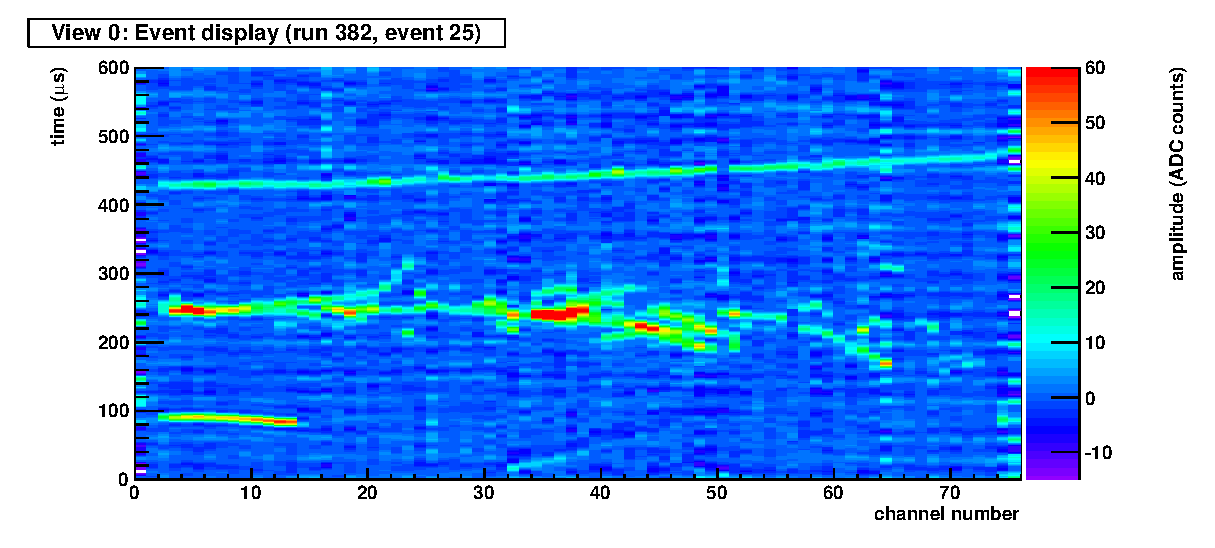
\includegraphics[width=1.0\hsize]{fig/Textbook.eps}
  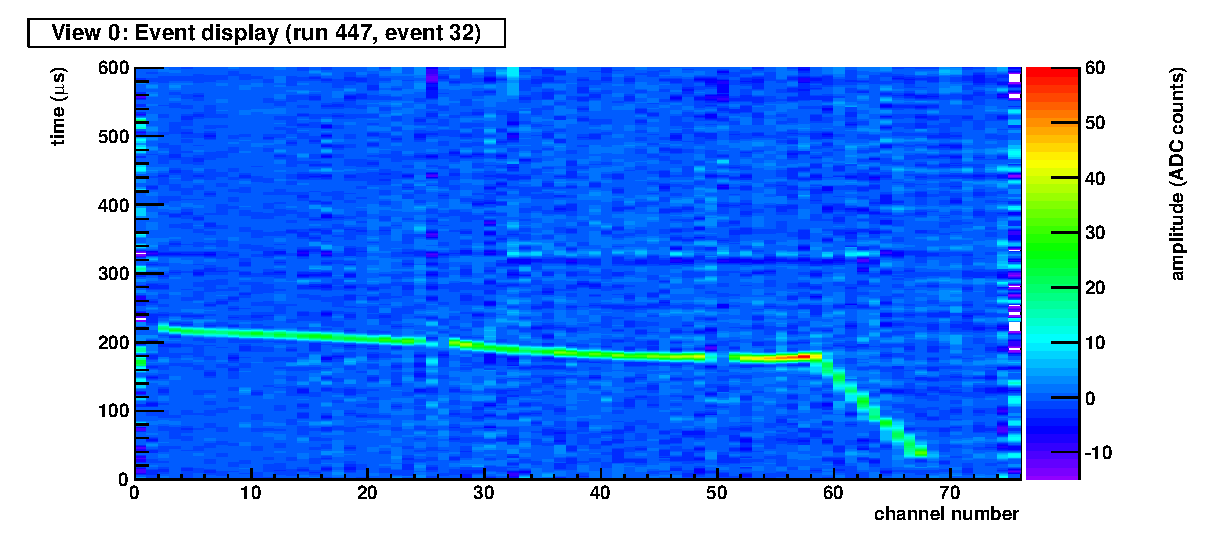
\includegraphics[width=1.0\hsize]{fig/Kmunu.eps}
 \end{center}
 \caption{Event display of 800 MeV/$c$ electron triggered event (top) accidentally overlapped with a proton and a pion,
   and Kaon 630 MeV/$c$ triggered event (bottom)}
 \label{Fig:Textbook}
\end{figure}


\subsubsection{Noise Reduction}
Dotted line in top plots of Fig.~\ref{Fig:FFT} shows raw waveform of the TPC signal
before applying any noise reduction. the waveform shown in this plot
are channel 13 in Fig.~\ref{Fig:Textbook} which are around the proton stopped point.
Signal-to-noise ratio for this particular case is poor and pion signal 
which is supposed to be t=400 $\mu$s is almost hidden by the noise. 
While time width of TPC signal is few $\mu$s which is determined by
drift time between anode and anode-grid, dominant noise component looks
higher frequency. To reduce such noises, we have applied FFT 
(Fast Flourier Transformation) filter to cut the high frequency component.
Bottom plot in Fig.~\ref{Fig:FFT} shows amplitude as a function of frequency
for the same event. This clearly shows dominant noise component with
$>$ 200 kHz has good separation with signal component ($<$ 100 kHz).
Solid line in top plot of Fig.~\ref{Fig:FFT} shows waveform after removing high frequency
($>$ 80 kHz) component by the FFT filter. Signal-to-noise ratio is dramatically
improved. On the other hand, we expect certain bias to the signal charge
measurement by this filter, and it will be discussed in Section x.

\begin{figure}[htbp]
 \begin{center}
  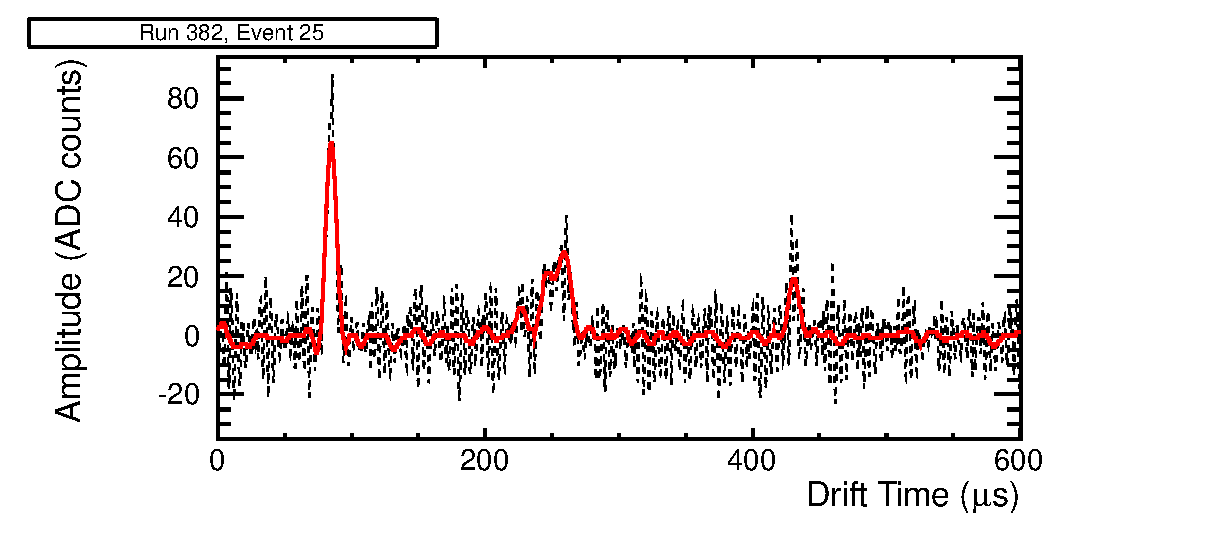
\includegraphics[width=1.0\hsize]{fig/beforeafterFFT.eps}
  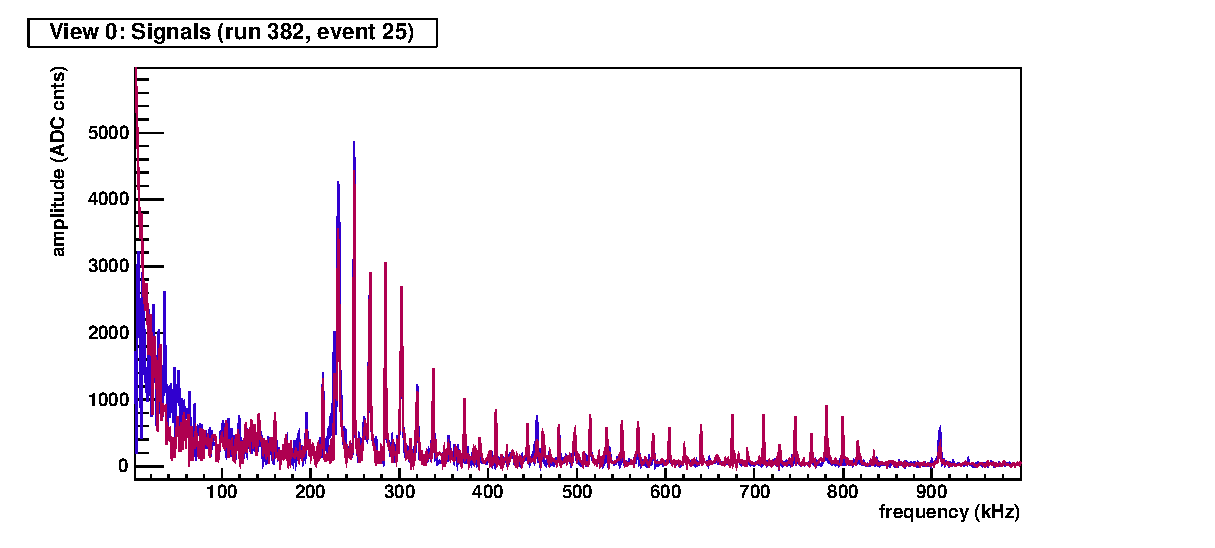
\includegraphics[width=1.0\hsize]{fig/FFT.eps}
 \end{center}
 \caption{Top: Typical TPC signal waveform before (dotted line) and after (solid line) applying FFT low pass filter with threshold of 80 kHz,
Bottom: FFT frequency amplitude distribution}
 \label{Fig:FFT}
\end{figure}


\subsubsection{Hit Finding/Clustering}
After noise reduction we find signal hits and create clusters associated to single tracks. 
Hit is defined as bump over given threshold in a channel. 
Threshold of hit finding is 6 ADC counts, which is about 2.5$\sigma$ from typical data noise level (as shown in Fig~\ref{Fig:FFT}) and keeping more than 99\% of Kaon hit finding efficiency in simulation.
% noise level from outside window of PhysicsOct55 (rms~2.49)
ADC count distribution is fitted by Gaussian plus step function to estimate the charge of hit in ADC $\times$ $\mu$s unit.
Fitting $\chi^2 < 3$ and $2.5<$~(time~width~of~hit)~$<8$~$\mu$s are required to remove noise hits further.
After finding all hits in an event, we construct cluster by merging adjacent hits. 
The example of hit finding and clustering using Fig~\ref{Fig:Textbook} event is shown in Fig~\ref{fig:Clustering}, which indicates reasonable hit and cluster findings. 

\begin{figure}[htbp]
 \begin{center}
  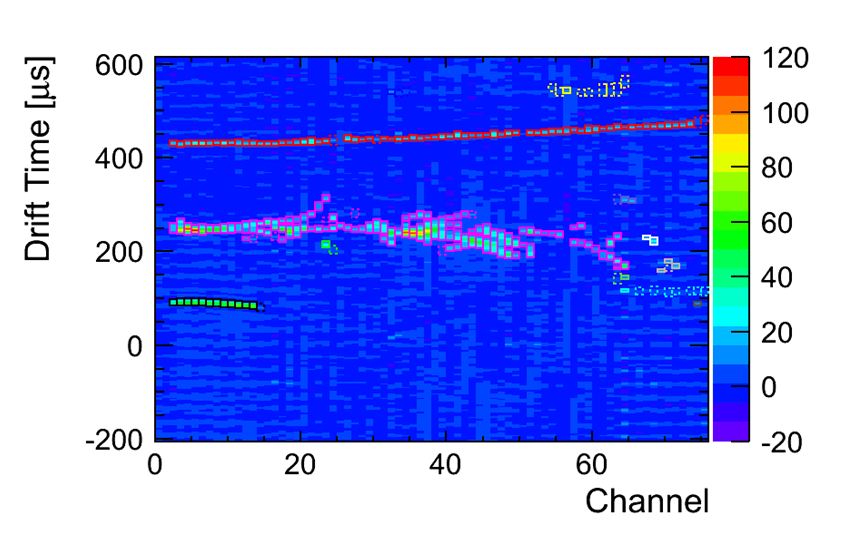
\includegraphics[width=1.0\hsize]{fig/clustering.eps}
 \end{center}
 \caption{Example of hit finding and clustering. A colored box corresponds to a hit and colors represent different clusters.}
 \label{fig:Clustering}
\end{figure}


%%%%%%%%%%%%%%%%%%%%%%%%%%%%%%%%%%%%%%%%%%%%%%%%%%
\subsection{Channel-by-Channel Calibration}
%%%%%%%%%%%%%%%%%%%%%%%%%%%%%%%%%%%%%%%%%%%%%%%%%%

Figure~\ref{fig:PionQvsCh} shows the hit charge as a function of 
the TPC channel number obtained from the 800 MeV/$c$ $\pi^+$ data. 
This figure is obtained from $\sim$300 events of well-selected Pion passing-through the TPC.
Gray-scale contours show hit charge distributions for
each channel and black points correspond to average of the hit charge distribution.  
Although we expect the energy deposition of the through-going pion to be uniform,
we observe relatively large channel dependence. 
This is mainly because of the distortion of the TPC drift field.
We use this average charge as channel-by-channel normalization scale.

\begin{figure}[htbp]
 \begin{center}
%  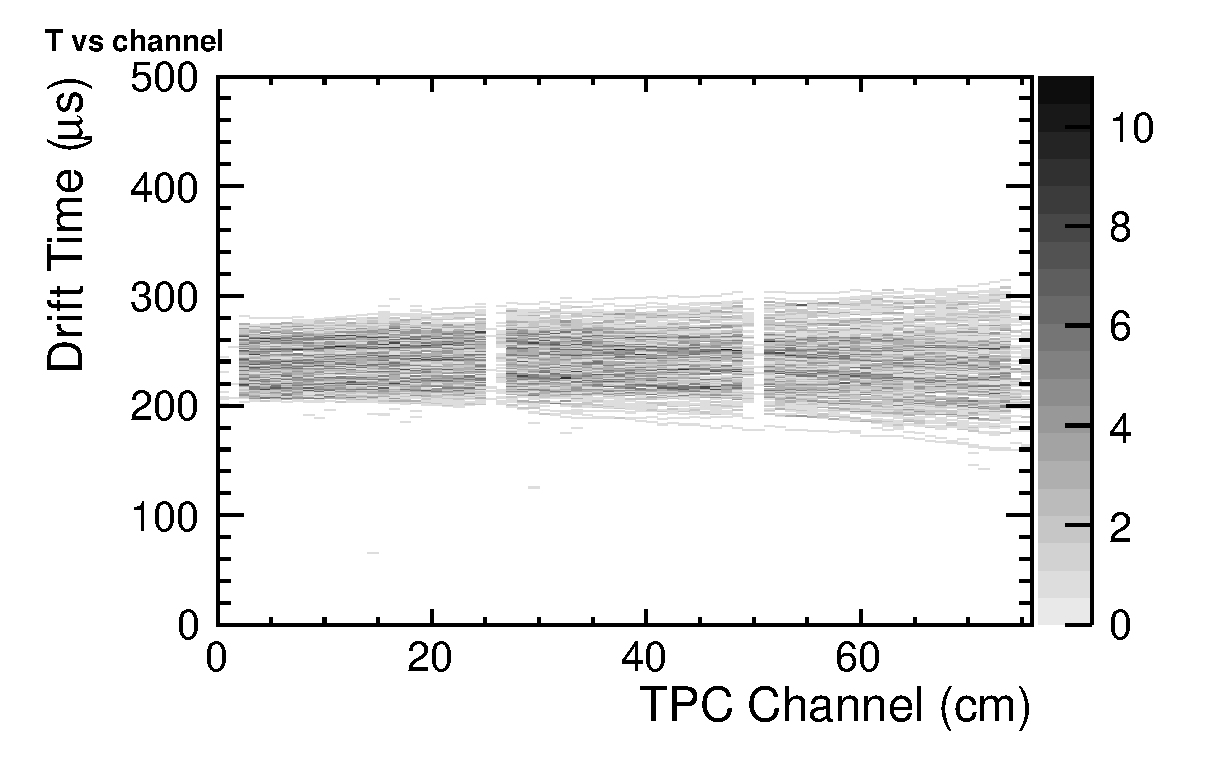
\includegraphics[width=0.8\hsize]{fig/PionTrack.eps}
  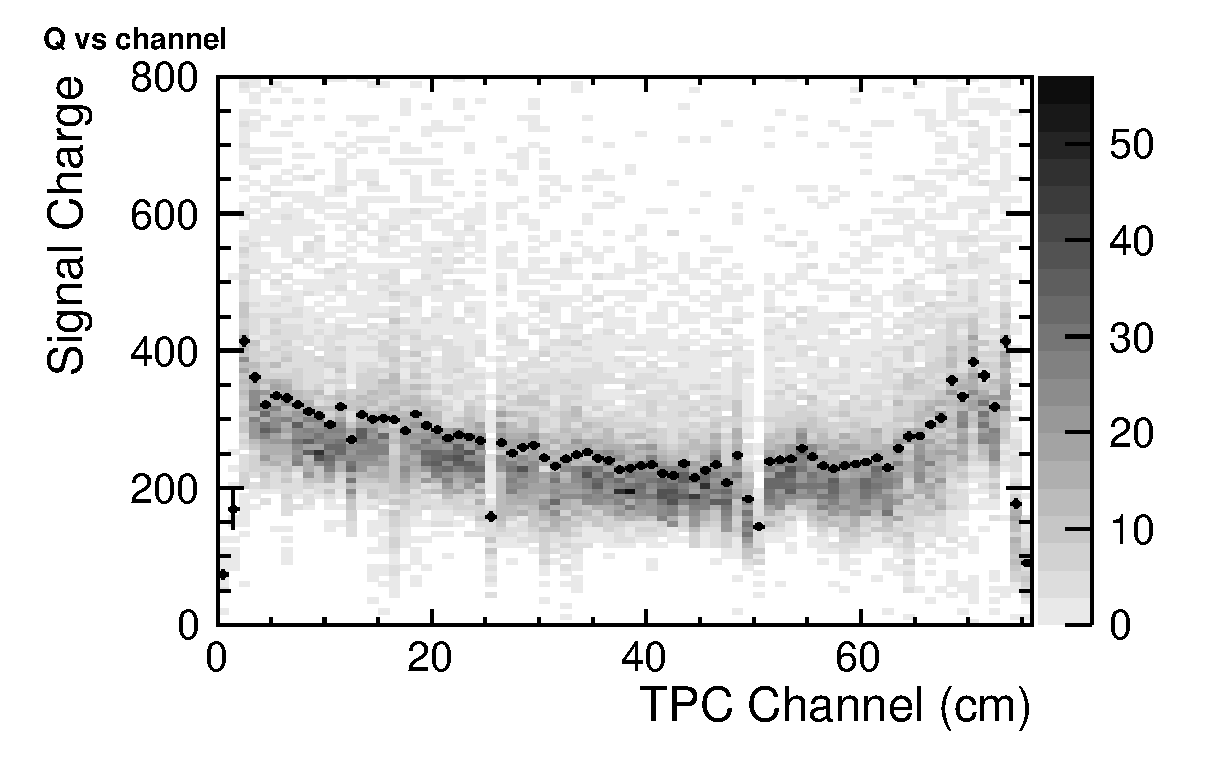
\includegraphics[width=1.0\hsize]{fig/PionQvsCh.eps}
 \end{center}
 \caption{800 MeV/c pion average hit charge}
 \label{fig:PionQvsCh}
\end{figure}

Figure~\ref{Fig:2DFieldMap} shows electric field of the TPC in V/cm which 
is calculated using a 2D FEM (Finite Element Method) package \cite{Ref:FEMTET},
where horizontal axis, vertical axis, and color strength 
correspond to the beam line direction, the drift direction, the electric field in V/cm, respectively.
Cathode, Anode, and Anode grid are located at of z=-200 mm, z=200 mm, and z=210 mm. respectively.
There are significant distortion of the electric field around 4 corners of the TPC fiducial volume,
and also around x=$\pm$120 mm where support structure of the Cathode and Anode grids exists.
We found this field distortion is the main cause of the
non-uniformity of the TPC response.

\begin{figure}[htbp]
 \begin{center}
  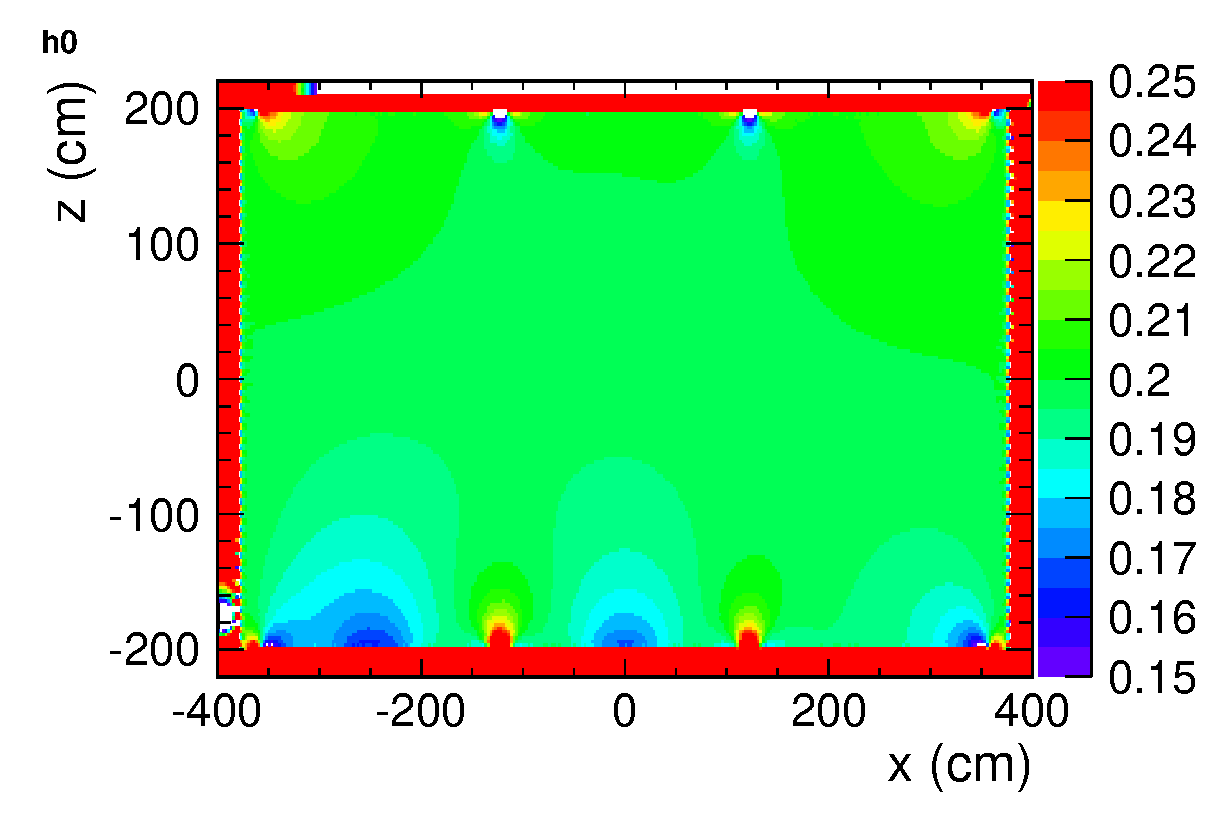
\includegraphics[width=1.0\hsize]{fig/2DFieldMap.eps}
 \end{center}
 \caption{Electric field map obtained with 2D FEM where
horizontal axis corresponds to the beam line direction,
and vertical axis corresponds to drift direction,
and color strength corresponds to electric field strength in V/cm.
}
 \label{Fig:2DFieldMap}
\end{figure}

%%%%%%%%%%%%%%%%%%%%%%%%%%%%%%%%%%%%%%%%%%%%%%%%%%
\subsection{Liquid Argon Purity}
%%%%%%%%%%%%%%%%%%%%%%%%%%%%%%%%%%%%%%%%%%%%%%%%%%

Attenuation of the drift electron depends on purity of LAr since electronegative impurities capture it \cite{purity}. 
Thus we need to apply correction to TPC signal charge according to the drift time.
We use cosmic ray events triggered by inner PMT at off-beam timing for measuring the LAr purity, and use this to correct the beam data.
Figure~\ref{fig:CosmicEvent} shows an event display of typical cosmic muon event crossing TPC channels.
The attenuation of readout charge depending on drift time is clearly seen in the right plot. 
We use multiple events to cancel Landau effect and apply channel response correction to estimate LAr purity.

\begin{figure}[htbp]
 \begin{center}
  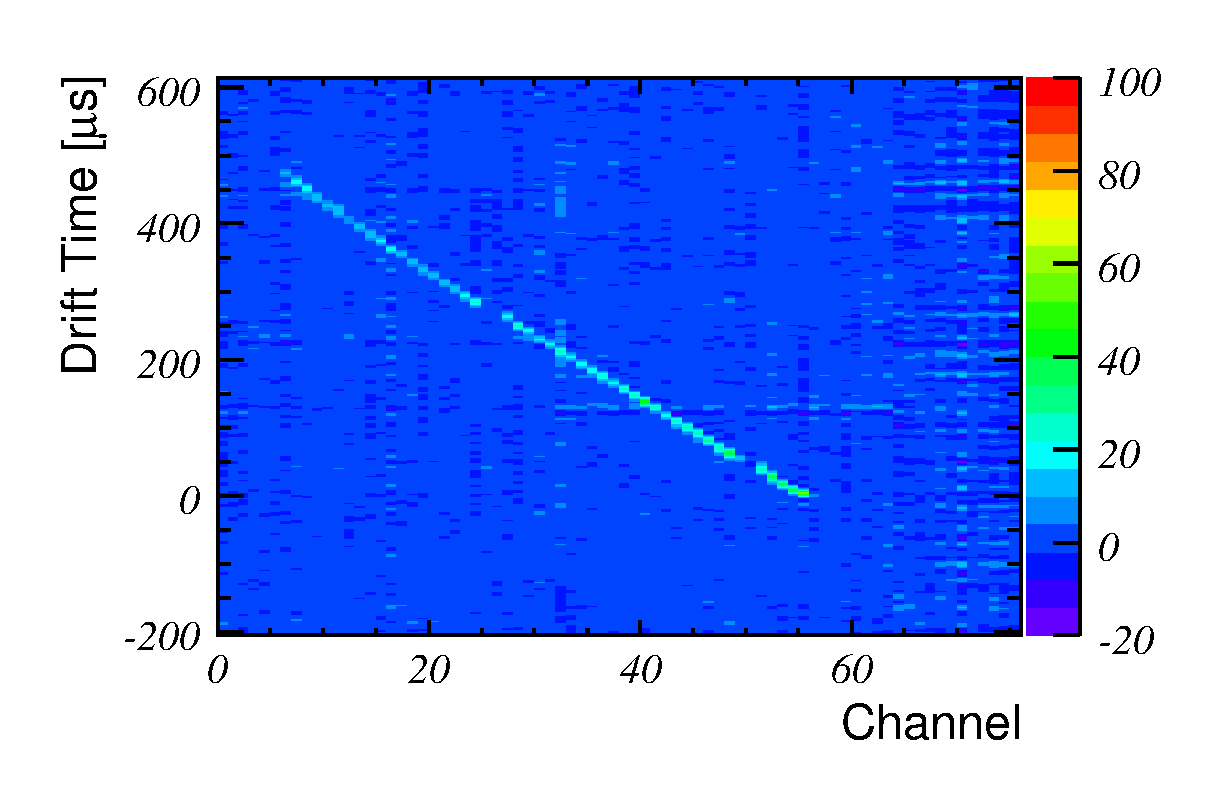
\includegraphics[width=0.49\hsize]{fig/cosmic68_ev258_display.eps}
  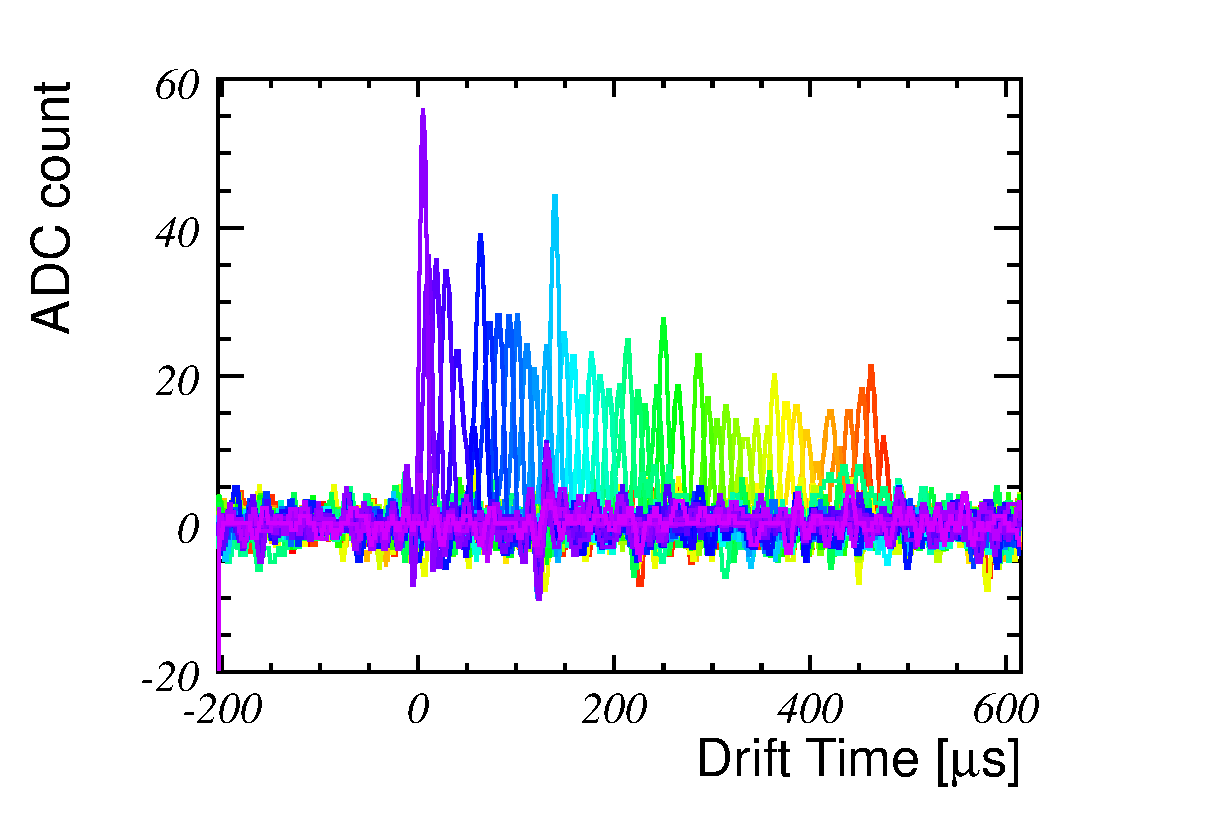
\includegraphics[width=0.49\hsize]{fig/cosmic68_ev258.eps}
 \end{center}
 \caption{Left: Typical cosmic muon event crossing TPC channels. Right: Charge deposit as a function of drift time.}
 \label{fig:CosmicEvent}
\end{figure}

We select cosmic ray event with more than 20 TPC channels which corresponds to zenith angle of more than $27^\circ$ and consistent with straight line by $\chi^2$ fit. 
%Readout charge is corrected for field distortion and projected to beam direction to correct injection angle.
We fit readout charge by Landau function in each drift time bin to estimate average charge deposit. 
%Figure~\ref{fig:tauExample} shows example of the average readout charge as a function of drift time which is fitted by exponential to obtain drift electron lifetime. 
%Realistic Monte Carlo simulation shows about 13\% (TBU) smaller lifetime estimation due to noise, field distortion, and FFT effects. 
%We correct output lifetime from these effects.
Figure~\ref{fig:CosmicPurity} shows an drift electron lifetime as a function of duration after initial LAr filling.
Drift electron lifetime was 600 $\mu$s at 60 hours, and 400 $\mu$s after 150 hours.
%Initial purity looks good, but the purity was slowly degrading while data taking period.
The degradation is possibly due to impurity from micro leak or out-gassing penetrating faster than purification by gas recirculation.
But we kept enough drift electron lifetime during data taking period.
The effects from noise, field distortion, and FFT give about 10\% (to be confirmed) of systematic uncertainty in LAr purity estimation.
%Since charge in simulation is calibrated using through-going $\pi$ data as described later and duration of analyzed beam data is short (about 30 hours), this uncertainty gives negligible effects (to be updated, show percentage) in beam data analysis. 

%\begin{figure}[htbp]
% \begin{center}
%  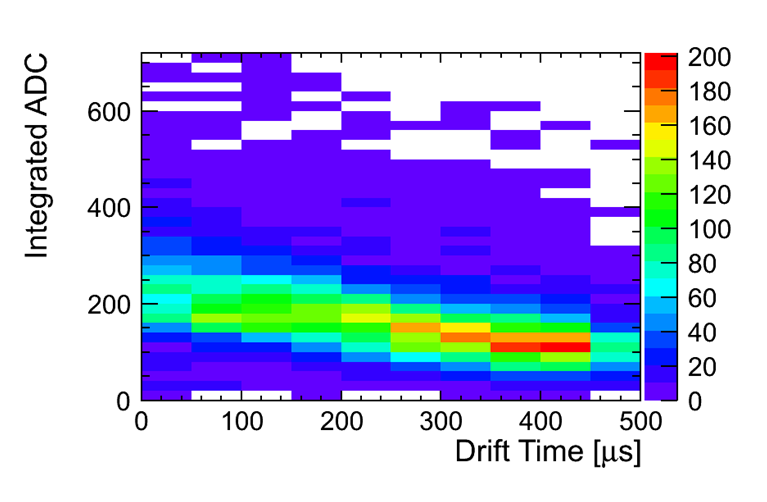
\includegraphics[width=0.45\hsize]{fig/chargeDep.eps}
%  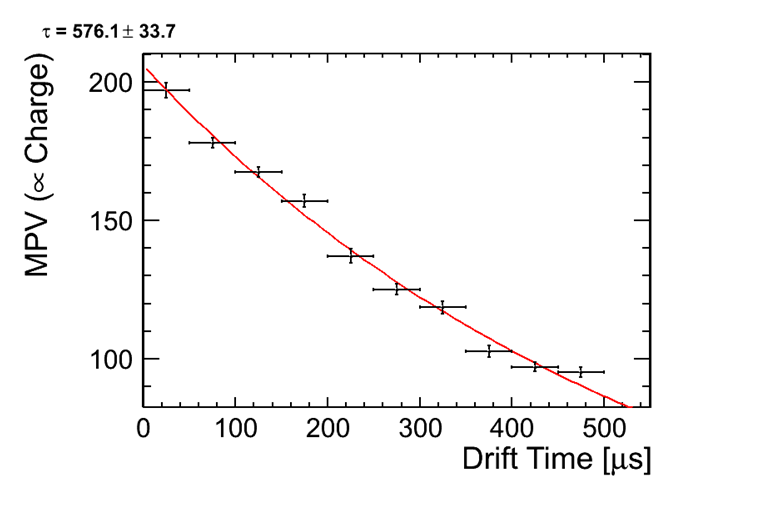
\includegraphics[width=0.45\hsize]{fig/tauExample.eps}
% \end{center}
% \caption{Left: Readout charge as a function of drift time. Readout charge in each drift time bin is fitted by landau function. Right: Average charge readout as a function of drift time which is fitted by exponential to estimate drift electron lifetime.}
% \label{fig:tauExample}
%\end{figure}

\begin{figure}[htbp]
 \begin{center}
  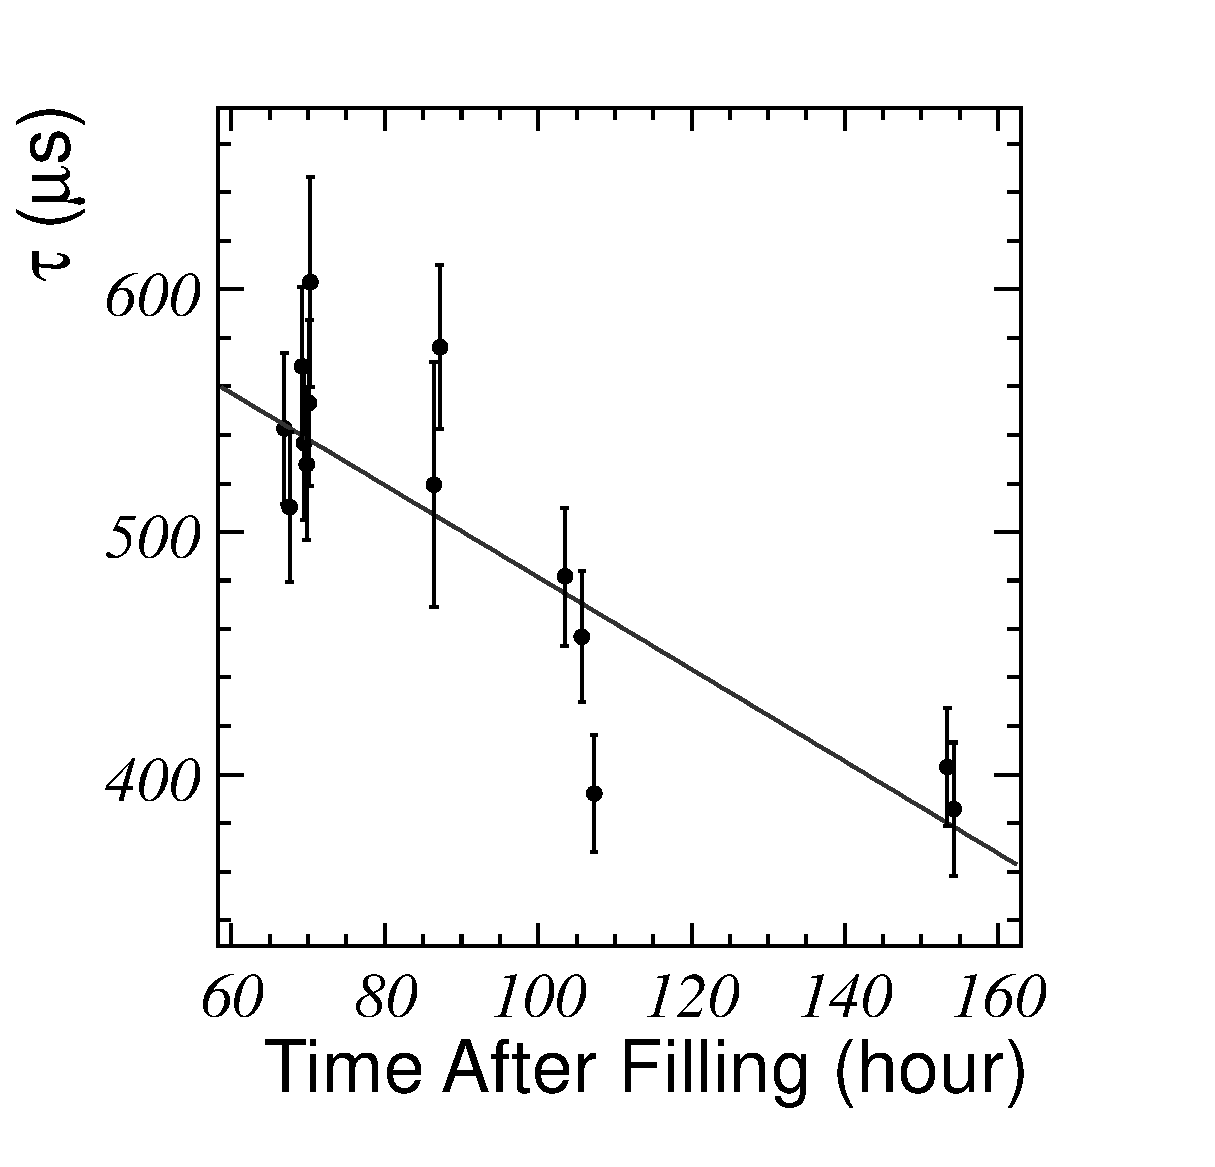
\includegraphics[width=1.0\hsize]{fig/tauHistory.eps}
 \end{center}
 \caption{Drift electron lifetime as a function of duration after initial LAr filling. The lifetime is used to correct the beam data.}
 \label{fig:CosmicPurity}
\end{figure}

\subsection{Cross Talk}

TBD

%Figure\ref{fig:cross_talk1} shows the signal wave form of stopped channel and the front channel of typical proton event.
%The signal wave form of stopped channel is differential form of the that of the front channel.
%Such signals are appeared at channel number 1 which cannot enter drifted ionization electron in electric power lines.
%One possibility which cause such a phenomenon is following process.
%The distance between anode channels is very short,
%so the influence of mutual capacitance become large
%and this capacitive coupling induce cross talk noise.
%This effect notably appears the channel where the difference of the charge between adjacent channels is large,
%such as the channel around stopped point of proton.
%Then, we implement this phenomenon in Monte Carlo Simulation
%by adding bipolar shape of the signal Gavin shape at adjacent channels.
%The area of the mountain of bipolar shape is 10.5\% of the area of signal Gaussian at each adjacent channel.
%The value of 10.5\% is determined by comparing the hit charge distribution at stopped channel between data and MC simulation.
%Figure\ref{fig:cross_talk2} shows hit charge distribution of stopped channel.
%Black is data and blue is MC simulation with cross talk red is MC simulation without cross talk.
%As fig\ref{fig:cross_talk2} shown, data and MC simulation with cross talk is good agreement,
%so the value of 10.5\% is reasonable.

\begin{figure}[htbp]
  \begin{center}
    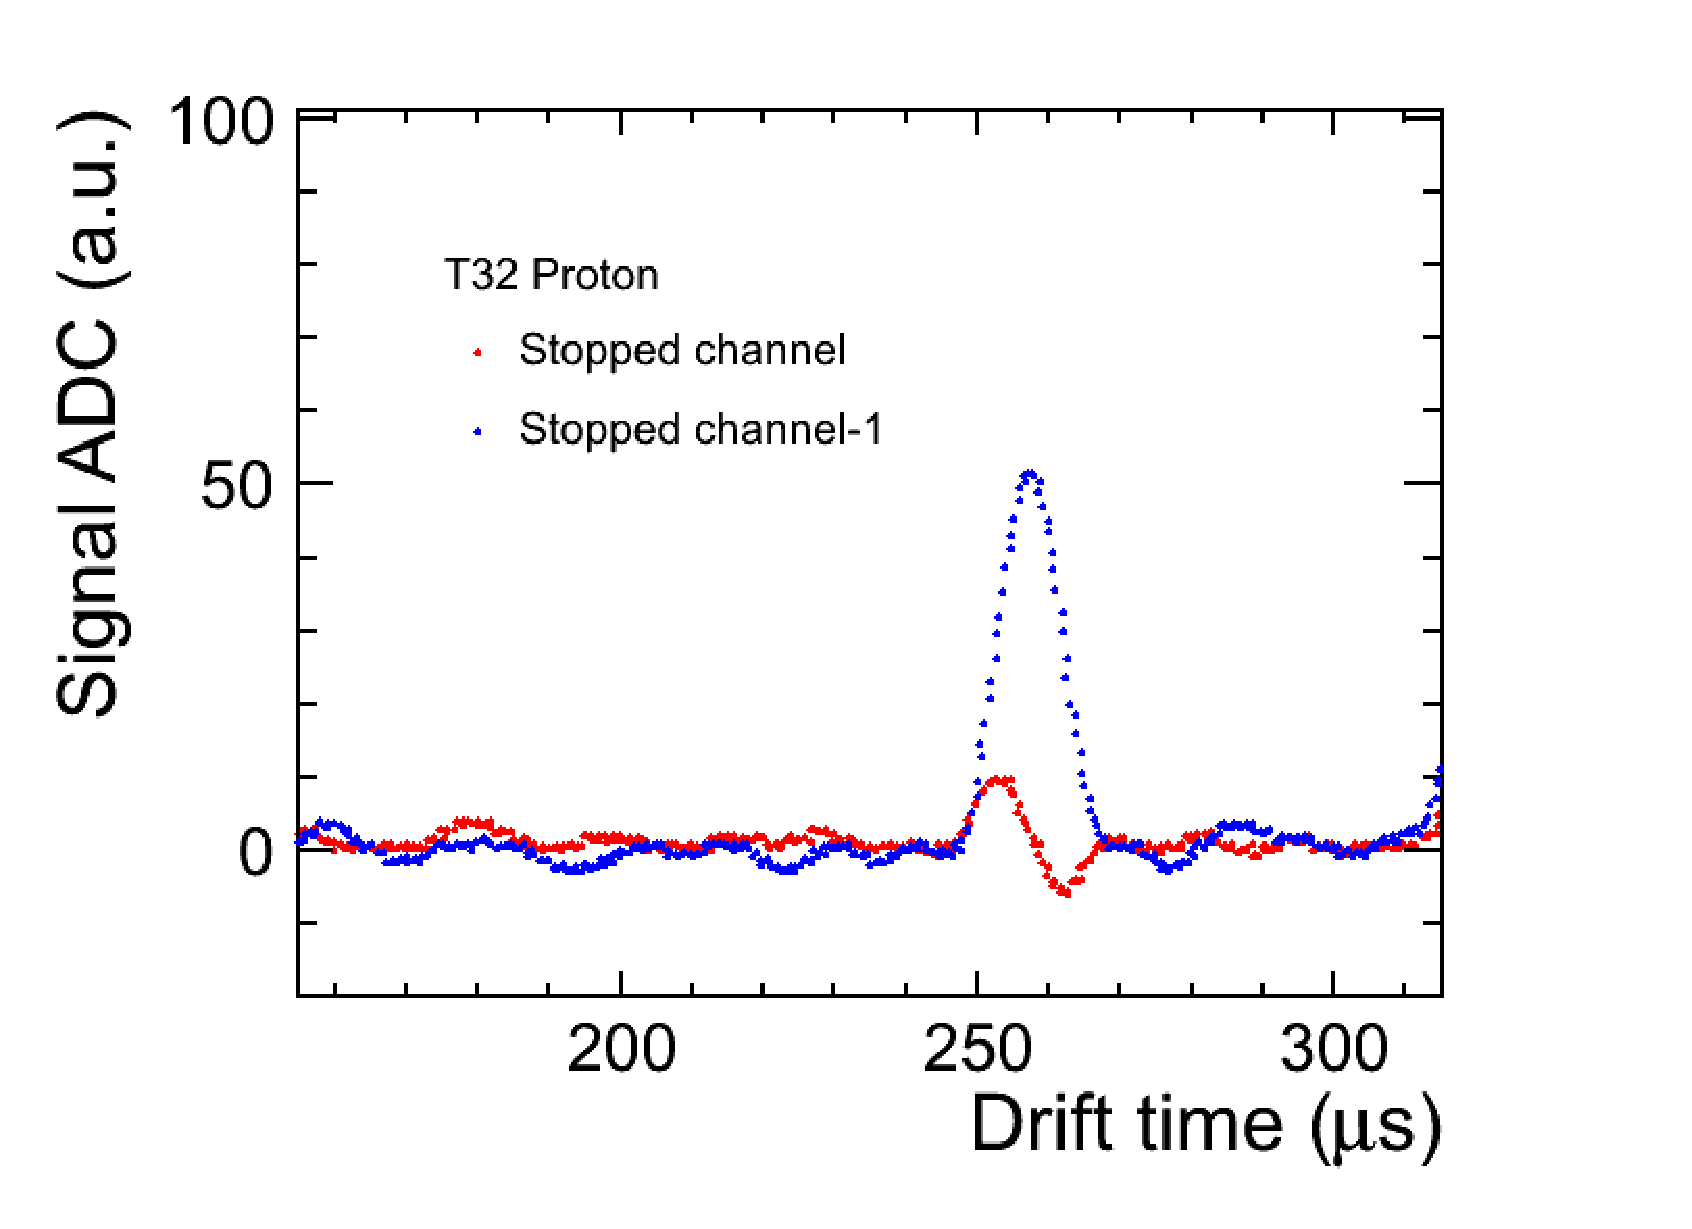
\includegraphics[width=1.0\hsize,clip]{fig/cross_talk_1.eps}
%    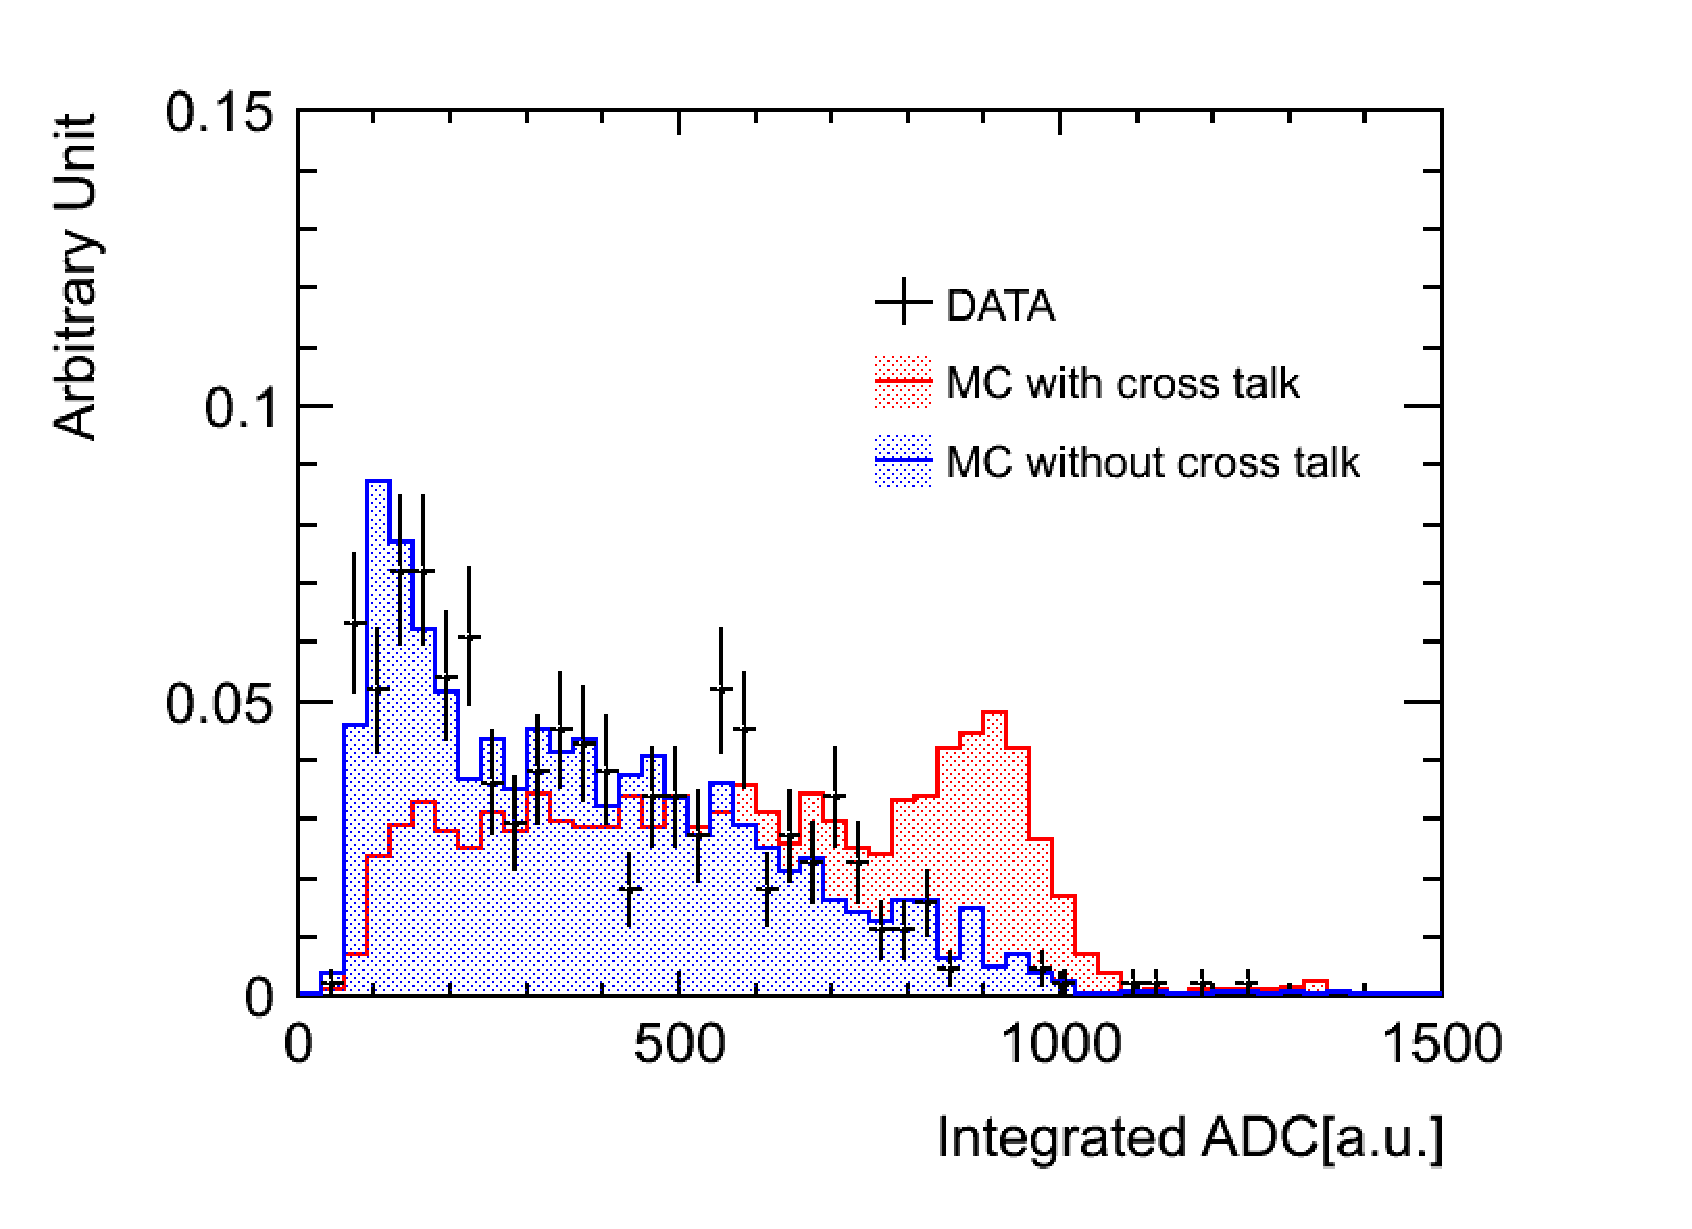
\includegraphics[width=0.45\hsize,clip]{fig/cross_talk_2.eps}
  \end{center}
  \caption{Left plot shows signal wave form of stopped channel and the front channel, 
    and right plot shows hit charge distribution of stopped channel}
  \label{fig:cross_talk1}
  \label{fig:cross_talk2}
\end{figure}
